% This work is licensed under the Creative Commons Attribution-NonCommercial 4.0 International License.
% To view a copy of this license, visit http://creativecommons.org/licenses/by-nc/4.0/
% or send a letter to Creative Commons, PO Box 1866, Mountain View, CA 94042, USA.

% !TEX TS-program = xelatex

\documentclass[../Main/chem331-notes.tex]{subfiles}
\begin{document}

\setcounter{section}{13}

\section{Many-electron atoms}
\subsection{Identical particles in quantum mechanics}
In this section we will explore the consequences of the fact that two or more particle are identical on their quantum mechanical behavior. Quantum mechanics takes the idea of two particles being identical very seriously.
From the point of view identical particles have the same physical properties (e.g. mass, charge). More importantly, quantum mechanics assumes that identical particle cannot be distinguished.
That is, there is no experiment we can perform that can distinguish particles of the same time, say two electrons.
The indistinguishability\mnote{Yes, a 20-letter word.} of identical particle must be reflected in the properties of the wave function that represents them.

Consider two identical particles and let us write the wave function as $\psi(x_1,x_2)$, where $x = (\mathrm{r},\sigma)$ collects both the position in space in the vector $\mathbf{r}$ and the spin variable $\sigma$.
The corresponding probability distribution is given by $P(x_1,x_2) = |\psi(x_1,x_2)|^2$.
To enforce the indistinguishability of the two particles we demand that the probability distribution is the same if we were to switch the way we label the particles. In this case only other possible way to label the particles is to switch $x_1$ and $x_2$. We can write this condition as
\begin{equation}
P(x_1,x_2) = P(x_2,x_1) \Rightarrow  |\psi(x_1,x_2)|^2 = |\psi(x_2,x_1)|^2.
\end{equation}
Note that this condition can be satisfied in two ways.
We can require the wave function with the particles exchanged to have the same value as the original wave function
\begin{equation}
\psi^\mathrm{B}(x_2,x_1) = +\psi^\mathrm{B}(x_1,x_2).
\label{eq:manyelectronatoms:bosons}
\end{equation}
Alternatively, we can require that the wave function with the permuted indices is minus the original wave function
\begin{equation}
\psi^\mathrm{F}(x_2,x_1) = - \psi^\mathrm{F}(x_1,x_2).
\label{eq:manyelectronatoms:fermions}
\end{equation}
This suggest that there are two fundamental behaviors of identical particles.
In the first case, when we permute the coordinates the sign of the wave function we get the original wave function with the plus sign (symmetric case). Particles that satisfy this condition are called \textbf{bosons}.
Bosons include particles that carry a fundamental force  like photons (electromagnetic force), gluons (strong force in quarks), and W and Z bosons (weak interaction), the Higgs boson (gives mass), and the yet-to-be-discovered graviton.
Particles for which the wave function changes sign (antisymmetric case) upon exchange of labels are called \textbf{fermions}. Fermions include particles like the electrons, quarks, as well as, composite particles like the proton.

The symmetry with respect to interchange of particles is also connected to the spin properties of particles. All bosons have integer values of the spin variable $s$. For example the photon has $s = 1$ while the Higgs has $s=0$. On the contrary, as we have already seen, fermions have half-integer spin, with the electron, proton, and neutron having $s = 1/2$.
The symmetry/antisymmetry properties of a wave function with respect to the exchange of two particles has very important physical consequences.
For example, fermions cannot occupy the same point is space\mnote{This statement has to account the fact that our definition of space also includes spin.} since if we evaluate the symmetry condition [Eq.~\eqref{eq:manyelectronatoms:fermions}] for $x_1 = x_2$ we get
\begin{equation}
\psi^\mathrm{F}(x_1,x_1) = - \psi^\mathrm{F}(x_1,x_1),
\end{equation}
which implies that $\psi^\mathrm{F}(x_1,x_1) = 0$.
This result is at the basis of Pauli's exclusion principle and the reason why we have chemical elements that behave so differently.
In the case of bosons, there is no problem with piling two or more bosons in the same point in space. Indeed at sufficiently low temperature bosons form what is called a Bose--Einstein condensate, in which all particles occupy the same quantum state.

\subsection{Wave functions for two electrons and determinants}
Suppose we have some approximate set of wave function for one electron, $\psi_n(x_1)$, how can we use these to build a fermion wave function that is  antisymmetric?
A straightforward way is to write the wave function as a product of the one-electron functions $\psi_n(x_1)$ that has been constructed to be antisymmetric
\begin{iequation}
\psi^\mathrm{F}(x_1,x_2) = \frac{1}{\sqrt{2}} \left[\psi_m(x_1) \psi_n(x_2) - \psi_m(x_2) \psi_n(x_1) \right].
\end{iequation}
You can easily verify that this wave function is antisymmetric with respect to the interchange of $x_1$ and $x_2$.
Note that if the two orbitals $\psi_m$ and $\psi_n$ are identical ($m = n$) this expression gives zero
\begin{equation}
\psi^\mathrm{F}(x_1,x_2) = \frac{1}{\sqrt{2}} \left[\psi_m(x_1) \psi_m(x_2) - \psi_m(x_2) \psi_m(x_1) \right] = 0.
\end{equation}
This is another manifestation of Pauli's exclusion principle.

This type of wave function is related to the concept of a \textbf{determinant}.
For a $2 \times 2$ matrix 
\begin{equation}
\mathbf{A} = 
\begin{pmatrix}
a & b \\
c & d
\end{pmatrix},
\end{equation}
the determinant $|\mathbf{A}|$ is defined as
\begin{equation}
|\mathbf{A}| = 
\begin{vmatrix}
a & b \\
c & d
\end{vmatrix}
=ad - bc.
\end{equation}
So we can rewrite the fermion wave function as
\begin{equation}
\psi^\mathrm{F}(x_1,x_2) = \frac{1}{\sqrt{2}}
\begin{vmatrix}
\psi_m(x_1) & \psi_m(x_2) \\
\psi_n(x_1) & \psi_n(x_2)
\end{vmatrix}.
\end{equation}
This quantity is often written in shorthand notation as
\begin{equation}
 \frac{1}{\sqrt{2}}
\begin{vmatrix}
\psi_m(x_1) & \psi_m(x_2) \\
\psi_n(x_1) & \psi_n(x_2)
\end{vmatrix} \leftrightarrow | \psi_m \psi_n \rangle.
\end{equation}

\subsection{The helium atom}
Now we can apply what we learned about wave functions for many fermions to the case of the helium atom.
We will continue to assume that the position of the nucleus is fixed to the origin.
This approximation (Born--Oppenheimer) is even more valid in the case of the helium atom since the mass of the nucleus is heavier than that of the proton.
The wave function of the helium atom is a function to the electron coordinates $\mathbf{r}_{1}$ and $\mathbf{r}_{2}$, as shown in Fig.~\ref{fig:manyelectronatoms:heliumcoordinates}. 
Using these coordinates, the Hamiltonian for the helium atom is given by
\begin{equation}
\hat{H} = 
\underbrace{
-\frac{\hbar^2}{2 m_2} \nabla^2_1 -\frac{\hbar^2}{2 m_2} \nabla^2_2
}_{\text{Kinetic energy}}
\;
\underbrace{
- \frac{1}{4\pi\epsilon_0} \frac{e^2 Z_\mathrm{He}}{r_1} - \frac{1}{4\pi\epsilon_0} \frac{e^2 Z_\mathrm{He}}{r_2}
}_{\text{Electron-nucleus potential energy}}
\underbrace{+
\frac{1}{4\pi\epsilon_0} \frac{e^2}{r_{12}},
 }_{\text{Electron-electron potential energy}}
\end{equation}
where $r_1 = |\mathbf{r}_1| = \sqrt{x_1^2 + y_1^2 + z_1^2}$ and $r_2  = |\mathbf{r}_2|= \sqrt{x_2^2 + y_2^2 + z_2^2}$ are the distance of electron 1 and 2 from the nucleus, respectively. The quantity $r_{12}$ is the distance between electron 1 and 2, defined as
\begin{equation}
r_{12}  = |\mathbf{r}_{12}| = \sqrt{(x_1 - x_2)^2 + (y_1 - y_2)^2 + (z_1 - z_2)^2}.
\end{equation}
\marginpar{
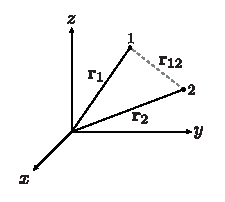
\includegraphics[width=1.5in]{../Figures/ManyElectronAtoms/HeliumCoordinates.pdf}
\captionof{figure}{Radial shell of radius $r$ and thickness $dr$.}
\label{fig:manyelectronatoms:heliumcoordinates}
}
The first term in the Hamiltonian is the sum of the kinetic energy for electron 1 and 2.
The second and third terms account for the attraction of the two electrons to the nucleus. Note that here we use a charge for the nucleus $q = e Z_\mathrm{He}$, where $Z_\mathrm{He} = 2$ is the atomic number of helium.
The last term accounts for the Coulomb repulsion (hence the plus sign) of the two negatively charged electrons.
This Hamiltonian can be written compactly in atomic units as
\begin{equation}
\hat{H} = -\frac{1}{2} \nabla^2_1 -\frac{1}{2} \nabla^2_2 - \frac{2}{r_1} - \frac{2}{r_2} + \frac{1}{r_{12}}.
\end{equation}

\subsection{Independent particle approximation}
The Hamiltonian for the helium atom is one of the first problems for which we cannot find an analytic solution.
The obstacle is that the last term in the Hamiltonian, the electron-electron repulsion term ($r_{12}^{-1}$) that couples the position of electron 1 and 2.
We have already seen a term like this in the case of the vibrational motion of a diatomics.\mnote{In this case it was the harmonic potential $\frac{1}{2} k x_{12}^2 = \frac{1}{2} k (x_1 - x_2)^2$.}
For diatomics we were able to find a coordinate transformation that allowed us to write the Hamiltonian as a sum of two Hamiltonian operators that acted on different variables ($r$ and $R$) and no term that coupled them.
In the case of the Helium atom, it is not possible to find such a transformation and we will have to resort to a variety of numerical methods.

In this section we will start with the independent particle approximation.
We initially consider the original helium atom Hamiltonian \textbf{without} the electron-electron repulsion  term
\begin{equation}
\hat{H}^{(0)} = -\frac{1}{2} \nabla^2_1 -\frac{1}{2} \nabla^2_2 - \frac{2}{r_1} - \frac{2}{r_2}.
\end{equation}
%We label this simplified Hamiltonian with the subscript ``(0)'' to note that this is a zeroth-order 
Rearranging the terms we can write this Hamiltonian as a sum of two independent Hamiltonians
\begin{equation}
\hat{H}^{(0)}  = \hat{H}_1 +  \hat{H}_2,
\end{equation}
where $\hat{H}_1$ is given by
\begin{equation}
\hat{H}_1 =  -\frac{1}{2} \nabla^2_1 - \frac{2}{r_1},
\end{equation}
and $\hat{H}_2$ is defined in a similar way.

The Hamiltonian $\hat{H}_1$ should look very familiar.
It has the same form of the hydrogen atom Hamiltonian, but with a potential of the form
\begin{equation}
V(r) = - \frac{Z}{r},
\end{equation}
where $Z$ is the nuclear charge and in this case is set equal to $Z = 2$.
The hydrogen atom wave functions can be easily extended to the case of a nucleus of an arbitrary charge.\mnote{This is often called a hydrogen-like atom.} The only difference is in the definition of the radial wave function
\begin{equation}
R_{n,l}(r,Z) = \sqrt{\frac{ (n-l-1)! }{ 2n (n+l)!} } \left(\frac{2Z}{n} \right)^{l + 3/2} r^l e^{-Zr/n} L_{n-l-1}^{2l+1}(2Zr/n).
\end{equation}
The energy of a hydrogen-like atom with nuclear charge $Z$ corresponding to a wave function $\psi_{n,l,m_l}$ is equal to\mnote{The symbol $E_\mathrm{h}$ stands for the energy measured in atomic units called the Hartree. $1 E_\mathrm{h} = 627.51$ kcal/mol = 27.211 eV.}
\begin{equation}
E_n = -\frac{Z^2}{2n^2} \, E_\mathrm{h}.
\end{equation}

Now we attempt to write a wave function for the helium atom.
Using a theorem on separable Hamiltonians that we proved before, we can write the wave function of the helium atom as a product of the eigenfunctions of $\hat{H}_1$ and $\hat{H}_2$.
The ground state will be the product of the ground state of each Hamiltonian, which is either an alpha 1s spin orbital [$\psi_\mathrm{1s}(\mathbf{r}_1) \alpha(\sigma_1)$] or a beta 1s spin orbital [$\psi_\mathrm{1s}(\mathbf{r}_1) \beta(\sigma_1)$].
Also, since the wave must be antisymmetric we need to use a determinant.
Note that we cannot the wave functions for electron 1 and 2 both be in the 1s spin orbital because this wave function is zero
\begin{equation}
\frac{1}{\sqrt{2}} \left[
\psi_\mathrm{1s}(\mathbf{r}_1) \alpha(\sigma_1)
\psi_\mathrm{1s}(\mathbf{r}_2) \alpha(\sigma_2)
-
\psi_\mathrm{1s}(\mathbf{r}_2) \alpha(\sigma_2)
\psi_\mathrm{1s}(\mathbf{r}_1) \alpha(\sigma_1)
\right] = 0.
\end{equation}

However, if we place one electron in an alpha 1s and one in a beta 1s spin orbital we get a viable wave function
\begin{equation}
\begin{split}
\Psi_0^{(0)} (\mathbf{r}_1,\sigma_1,\mathbf{r}_2,\sigma_2) 
& =
\frac{1}{\sqrt{2}} \left[
\psi_\mathrm{1s}(\mathbf{r}_1) \alpha(\sigma_1)
\psi_\mathrm{1s}(\mathbf{r}_2) \beta(\sigma_2)
-
\psi_\mathrm{1s}(\mathbf{r}_2) \alpha(\sigma_2)
\psi_\mathrm{1s}(\mathbf{r}_1) \beta(\sigma_1)
\right] \\
& = 
\frac{1}{\sqrt{2}} 
\psi_\mathrm{1s}(\mathbf{r}_1)
\psi_\mathrm{1s}(\mathbf{r}_2)
\left[
\alpha(\sigma_1)
\beta(\sigma_2)
-
\alpha(\sigma_2)
\beta(\sigma_1)
\right].
\end{split}
\end{equation}
In the second line, we have separated the terms that depend on the position of the electrons [$\psi_\mathrm{1s}(\mathbf{r}_1)
\psi_\mathrm{1s}(\mathbf{r}_2)$] from terms that depend only on spin wave functions.
These two parts have different symmetry properties.
The spatial part of the ground state wave function for helium is symmetric with respect to the exchange of electron 1 and 2
\begin{equation}
\psi_\mathrm{1s}(\mathbf{r}_1)
\psi_\mathrm{1s}(\mathbf{r}_2)
=\psi_\mathrm{1s}(\mathbf{r}_2)
\psi_\mathrm{1s}(\mathbf{r}_1).
\end{equation}
Instead, the spin part is antisymmetric
\begin{equation}
\alpha(\sigma_1)
\beta(\sigma_2)
-
\alpha(\sigma_2)
\beta(\sigma_1)
=
- \left[
\alpha(\sigma_2)
\beta(\sigma_1)
-
\alpha(\sigma_1)
\beta(\sigma_2)
\right].
\end{equation}
When these two parts are multiplied together, we obtain a wave function that is overall antisymmetric.

Writing all these indices is a bit tedius, so we will use another notation that is somewhat shorter and write the ground state of the helium atom as
\begin{equation}
\Psi_0^{(0)} (\mathbf{r}_1,\sigma_1,\mathbf{r}_2,\sigma_2)
= |\underbrace{\psi_\mathrm{1s} \alpha}_{1} \, \underbrace{\psi_\mathrm{1s}  \beta}_{2}|.
\end{equation}
Since electrons are indistinguishable, we do not have to worry about explicitly indexing them when we want to represent a Slater determinant.
So we will implicitly understood that each spin orbital in this representation indicates a different electron.
The energy of this state can be computed as the sum of the eigenvalues of the two states that enter the Slater determinant
\begin{equation}
E^{(0)} = 2 E_1 = -2 \frac{2^2}{2} = - 4 \,E_\mathrm{h}.
\end{equation}
Note that this value is quite different from the experimentally determined energy of the helium atom
\begin{iequation}
E_\mathrm{exp} = - 2.9033 \,E_\mathrm{h}.
\end{iequation}
The independent electron approximation is ca. 38\% below the exact answer!
This result shows that the assumption that electrons behave independently is not particularly good.
Our next step will be to try to account for the electron-electron repulsion term.

\subsection{Excited states of the helium atom}
The wave function $|\psi_\mathrm{1s} \alpha \, \psi_\mathrm{1s}  \beta|$ corresponds to the (1s)$^2$ electrons configuration and is the only determinant we can write using the 1s orbitals of helium.
States with higher energy can be found by finding all nonzero determinants for electronic configurations in which electrons are excited to higher energy orbitals.

In the case of the  (1s)$^1$(2s)$^1$ configuration, we can write four nonzero Slater determinants
\begin{align}
\Psi_1^{(0)} & = |\psi_\mathrm{1s} \alpha \, \psi_\mathrm{2s}  \alpha|, \\
\Psi_2^{(0)} & = |\psi_\mathrm{1s} \alpha \, \psi_\mathrm{2s}  \beta|, \\
\Psi_3^{(0)} & = |\psi_\mathrm{1s} \beta \, \psi_\mathrm{2s}  \alpha|, \\
\Psi_4^{(0)} & = |\psi_\mathrm{1s} \beta \, \psi_\mathrm{2s}  \beta|.
\end{align}
These four determinants correspond to four electronic states, which are degenerate when we ignore the electron repulsion term in the Hamiltonian. Their energy is
\begin{equation}
E^{(0)} = E_1 + E_2 = -\frac{4}{2} -\frac{4}{8} = - 2.5 \,E_\mathrm{h}.
\end{equation}

%We can also 
%When we deal with more than one electron, it is important to label the operators with the index of the electrons on which they act. The equations that express the properties of spin eigenfunctions then become
%\begin{align}
%\hat{s}^2(j) \alpha(j)  = \frac{3}{4}\hbar^2 \alpha(j) \quad\quad
%\hat{s}^2(j) \beta(j)  = \frac{3}{4}\hbar^2 \beta(j),
%\end{align}
%and 
%\begin{align}
%\hat{s}_z(j) \alpha(j)  = \frac{1}{2}\hbar \alpha(j) \quad\quad
%\hat{s}_z(j) \beta(j)  = -\frac{1}{2}\hbar \beta(j),
%\end{align}
%where the index $j$ labels the electron ($j$ = 1 or 2), and ``$(j)$'' indicates which electron does an operator act on.
%For convenience we label the spin functions also with ``$(j)$'' instead of the more lengthy ``$(\sigma_j)$''.
%Here we use lower case letters to indicate operators that act only on one electron.

To understand the properties of these states we need to introduce total angular momentum and spin operators.
For example, for two electrons, the projection of angular momentum on the $z$ axis is given by the sum of the $\hat{L}_{z}$ operator that acts on electron 1, $\hat{L}_{z}(1)$, plus the same operator that acts on electron 2, $\hat{L}_{z}(2)$,
\begin{equation}
\hat{L}_z = \hat{L}_{z}(1) + \hat{L}_{z}(2).
\end{equation}
The total angular momentum squared is also defined as
\begin{equation}
\hat{L}^2 = \left[ \hat{\mathbf{L}}(1) + \hat{\mathbf{L}}(2) \right]^2.
\end{equation}
The eigenvalues of $\hat{L}^2$ are $\hbar^2 L(L+1)$, where $L$ is the quantum number for the total angular momentum squared.
 The eigenvalues of this operator $\hat{L}_z$ are $\hbar M_L$, where the quantum number $M_L$ can take all integer values between $L$ and $-L$ 
\begin{iequation}
M_L = L, L -1, \ldots, 0, \ldots, -L + 1, -L.
\end{iequation}
To find the value of $M_L$ for a determinant, we just sum up all the values of $m_l$ for each orbital occupied by an electron
\begin{iequation}
M_L = \sum_i m_l(i),
\end{iequation}
where $m_l(i)$ is the value of $m_l$ for the orbital of the $i$th electron and the sum runs over all the orbitals in a determinant.
All the four determinants in the (1s)$^1$(2s)$^1$ configuration have $M_L = 0$ because both the 1s and 2s orbitals have $m_l = 0$.
%\begin{equation}
%\hat{L}_z  |\psi_\mathrm{1s} \alpha \, \psi_\mathrm{2s}  \alpha| = 
% \hat{L}_{z}(1)|\psi_\mathrm{1s} \alpha \, \psi_\mathrm{2s}  \alpha|  + 
% \hat{L}_{z}(2)|\psi_\mathrm{1s} \alpha \, \psi_\mathrm{2s}  \alpha| 
% = 0 + 0 = 0 |\psi_\mathrm{1s} \alpha \, \psi_\mathrm{2s}  \alpha|.
%\end{equation}
This means that the four excited determinants have $L = 0$. Otherwise, we should have found some states with $M_L \neq 0$.
Physically, this means that all states have total angular momentum equal to zero.
These states behave like the s states of the hydrogen atom and so we indicated them with the symbol ``S''.

This analysis can be extended to spin. We find that the total spin squared operator $\hat{S}^2$ has eigenvalues equal to $\hbar^2 S(S+ 1)$, where $S$ is a quantum number analogous to $s$ for one electron. The projection of spin on the $z$ axis is instead $\hat{S}_z$, and its eigenvalues are $\hbar M_S$, where
\begin{iequation}
M_S = S, S -1, \ldots, 0, \ldots, -S + 1, -S.
\end{iequation}
For a given value of $S$ there are $2S +1$ possible values of $M_S$. Therefore call the number $2S +1$ the \textbf{spin multiplicity} of a state.
Every Slater determinant is an eigenfunction of $\hat{S}_z$, and it is very easy to find the quantum number $M_S$, it is just given by
\begin{iequation}
M_S = \frac{1}{2} (\text{number of alpha electrons} - \text{number of beta electrons}).
\end{iequation}


For our four determinants we have
\begin{align}
\hat{S}_z \Psi^{(0)}_1 & = \hat{S}_z |\psi_\mathrm{1s} \alpha \, \psi_\mathrm{2s}  \alpha| = \hbar \Psi^{(0)}_1, \\
\hat{S}_z \Psi^{(0)}_2 & = \hat{S}_z  |\psi_\mathrm{1s} \alpha \, \psi_\mathrm{2s}  \beta| = 0, \\
\hat{S}_z \Psi^{(0)}_3 & = \hat{S}_z  |\psi_\mathrm{1s} \beta \, \psi_\mathrm{2s}  \alpha| = 0, \\
\hat{S}_z \Psi^{(0)}_4 & = \hat{S}_z  |\psi_\mathrm{1s} \beta \, \psi_\mathrm{2s}  \beta| = -\hbar \Psi^{(0)}_4.
\end{align}

%All these states are eigenstates of the operator $\hat{L}_z$ with eigenvalue equal to zero


%The total projection of spin onto the $z$ axis is the sum of the $\hat{s}_{z}$ operator that acts on electron 1, $\hat{s}_{z}(1)$, plus the same operator that acts on electron 2, $\hat{s}_{z}(2)$
%Note that we use the upper case letter $S$ to indicate a \textbf{total} spin operator that acts on both electron 1 and 2.
%The total spin squared operator is a bit more complicated and contains contributions from the $x$, $y$, and $z$ components of the lower case spin operators
%\begin{equation}
%\hat{S}^2 = \hat{s}^2(1) + \hat{s}^2(2) + 2 [\hat{s}_{x}(1) \hat{s}_{x}(2) + \hat{s}_{y}(1) \hat{s}_{y}(2) + \hat{s}_{z}(1) \hat{s}_{z}(2)].
%\end{equation}

%\begin{problemenum}
%\item Show that the functions $\alpha(1)\alpha(2)$ and  $\beta(1)\beta(2)$ are eigenfunctions of the $\hat{S}_z$ operator.
%What is the corresponding eigenvalue?
%\begin{advice}
%Note that each lower case operator acts only on one electron coordinate. For example,
%\begin{equation}
%\hat{s}_z(2) \alpha(1)\alpha(2)
%= \alpha(1) \hat{s}_z(2) \alpha(2)
%= +\frac{\hbar}{2}  \alpha(1) \alpha(2).
%\end{equation}
%\end{advice}
%
%\item Using the fact that
%\begin{equation}
%\begin{split}
%\hat{s}_x(j) \alpha(j)  = +\frac{\hbar}{2} \beta(j) \quad
%\hat{s}_y(j) \alpha(j)  = +\frac{i\hbar}{2} \beta(j) \quad
%\hat{s}_z(j) \alpha(j)  = +\frac{\hbar}{2} \alpha(j) \\
%\hat{s}_x(j) \beta(j)  = +\frac{\hbar}{2} \alpha(j) \quad
%\hat{s}_y(j) \beta(j)  = -\frac{i\hbar}{2} \alpha(j) \quad
%\hat{s}_z(j) \beta(j)  = -\frac{\hbar}{2} \beta(j)
%\end{split}
%\end{equation}

So we find the following values of $M_S$: 1, 0, 0, $-1$. This is compatible with group of three states with $S =1$, which gives $M_S = 1, 0, -1$ and one state with $S = 0$ and $M_S = 0$.
We indicate the three states with $S =1$ and $L = 0$ with the symbol $^{3}S$ (read as triplet s), where the ``3'' is the spin multiplicity $2S +1 = 3$. In the same way, we indicate the state with $S =0$ and $L = 0$ with the symbol $^{1}S$ (read as singlet s).

\subsection{The effects of electron repulsion on the ground state}
We have seen that when we ignore the effects of electron repulsion we get an energy for the ground state that is too low and we predict that the first set of excited states are degenerate.
An approximate way to account for the effect of electron repulsion is to reintroduce the electron-electron repulsion term using perturbation theory.
The first-order correction to the energy from perturbation theory to energy of the ground state is equal to
\begin{equation}
\begin{split}
E_0^{(1)} = & \int [\Psi_0^{(0)}]^* \frac{1}{r_{12}} \Psi_0^{(0)} d\mathbf{r}_1 d\sigma_1 d\mathbf{r}_2 d\sigma_2  \\
= &
\int d\mathbf{r}_1 d\mathbf{r}_2 
\psi_\mathrm{1s}^*(\mathbf{r}_1)
\psi_\mathrm{1s}^*(\mathbf{r}_2)
\frac{1}{r_{12}}
\psi_\mathrm{1s}(\mathbf{r}_1)
\psi_\mathrm{1s}(\mathbf{r}_2) \\
= &
\int d\mathbf{r}_1 d\mathbf{r}_2 
\frac{|\psi_\mathrm{1s}(\mathbf{r}_1)|^2 |\psi_\mathrm{1s}(\mathbf{r}_2)|^2}{r_{12}}.
\end{split}
\end{equation}
In doing the integral, the spin part gives a contribution equal to one leaving an integral in the spatial coordinates $\mathbf{r}_1$ and $\mathbf{r}_2$.
The final integral has a classical interpretation. The square of a wave function is a probability density, so the term $|\psi_\mathrm{1s}(\mathbf{r}_1)|^2$ can regarded as the density of the electron charge for the 1s orbital, which we indicate with $\rho_\mathrm{1s}(\mathbf{r}_1)$. Therefore we can rewrite the integral as the classical Coulomb interaction energy of two charge distributions
\begin{iequation}
E^{(1)} = \int d\mathbf{r}_1 d\mathbf{r}_2 
\frac{\rho_\mathrm{1s}(\mathbf{r}_1)\rho_\mathrm{1s}(\mathbf{r}_2)}{r_{12}}.
\end{iequation}
This integral can be evaluated analytically for any given value of $Z$ and is equal to
\begin{equation}
E^{(1)} = \frac{5}{8}Z.
\end{equation}
In our treatment of the helium atom we use the wave functions that correspond to $Z = 2$ and this gives a first-order corrected energy equal to
\begin{equation}
E^{(0)} + E^{(1)} = -4 + \frac{5}{4} = -\frac{11}{4} = -2.75 \,E_\mathrm{h}.
\end{equation}
This number is in much better agreement with the experimental value ($-2.9033 \,E_\mathrm{h}$).

\subsection{Improving upon perturbation theory: variational minimization}
Our energy from perturbation theory can be further improved. 
Note that when we solved for the ground state wave function neglecting the electron-electron repulsion, we obtained a wave function $\Psi_0^{(0)}$ that was built from orbitals of independent electrons that interact only with the nucleus.
The electron-electron interaction, however, will push electrons apart from each other, giving us orbitals that are slightly different than those of the He$^+$ ion.

To improve our answer we will use the variational principle. This states that any normalized trial wave function $\tilde{\psi}$, has an energy expectation value that is greater than that of the true ground state. For a wave function that depends on only one coordinate ($x$) the variational principle is
\begin{equation}
\int \tilde{\psi}^*(x) \hat{H} \tilde{\psi}(x) \, dx \geq E_0 = \int \psi_0^*(x) \hat{H} \psi_0(x) \, dx,
\end{equation}
where $E_0$ and $\psi_0$ are the ground state energy and eigenfunction, respectively.
The variational principle gives us the right to seek a more accurate wave function by minimizing the value of the expectation value of the energy
\begin{equation}
E[\tilde{\psi}] = \int \tilde{\psi}^*(x) \hat{H} \tilde{\psi}(x) \, dx,
\end{equation}
because we are always guaranteed that this energy will be greater than or equal to the true ground state energy.
When we find the true minimum of $E[\tilde{\psi}]$ we are also guaranteed to have found the exact ground state solution of the ground state.

There are two ways we can improve our wave function for the helium atom.
First, we can still approximate the wave function with only one Slater determinant, but seek orbitals that keep into account the electron repulsion term.
This approach is called \textbf{Hartree--Fock theory}.
In Hartree--Fock theory the wave function is given by one Slater determinant
\begin{equation}
\Psi_\mathrm{HF} = |\psi_\mathrm{HF} \alpha \, \psi_\mathrm{HF} \beta|,
\end{equation}
where $\psi_\mathrm{HF}(\mathbf{r})$ is an optimized orbital that minimizes the energy of the wave function $\Psi_\mathrm{HF}$.
A numerical minimization of the energy yields the following result
\begin{equation}
E_\mathrm{HF} = \int \Psi^*_\mathrm{HF} \hat{H} \Psi_\mathrm{HF} = -2.8615 \, E_\mathrm{h}.
\end{equation}
This result is much closer to the experimental value, but the difference is of the order of $0.04$ $E_\mathrm{h}$, that is ca. 26 kcal mol$^{-1}$ or 1.1 eV.

We can do better if we allow the wave function to be a linear combination of determinants. This approach is known as \textbf{configuration interaction} and it is formally exact but much more expensive than Hartree--Fock theory. Configuration interaction is based on a wave function formed from a linear combination of Slater determinants
\begin{equation}
\Psi_\mathrm{CI} = \sum_{n=0}^\infty \Psi_n c_n,
\end{equation}
where the quantity $\Psi_n$ is a Slater determinant and the parameters $c_n$ must be optimized numerically.
The energy obtained by minimizing the energy of the wave function $\Psi_\mathrm{CI}$ is equal to\mnote{Both the Hartree--Fock and configuration interaction calculations reported here use a finite basis set (cc-pVQZ). This approximation introduces additional (small) errors.}
\begin{equation}
E_\mathrm{CI} = \int \Psi^*_\mathrm{CI} \hat{H} \Psi_\mathrm{CI} = -2.9024 \, E_\mathrm{h}.
\end{equation}
This answer is in very good agreement with the experimental result.
These calculations neglect small effects as corrections to the Born--Oppenheimer (clamped nucleus) approximation and relativistic effects.

\subsection{The effects of electron repulsion on the (1s)$^1$(2s)$^1$ excited states}
To understand the impact of electron correlation on the $^1$S and $^3$S excited states of helium we will analyze the structure of the wave function.
The $\Psi_1^{(0)} = |\psi_\mathrm{1s} \alpha \, \psi_\mathrm{2s}  \alpha|$ determinant corresponds to a wave function with antisymmetric spatial part and symmetric spin part
\begin{equation}
\begin{split}
\Psi_1^{(0)} & = 
 \frac{1}{\sqrt{2}}
\begin{vmatrix}
\psi_\mathrm{1s}(1) \alpha(1) & \psi_\mathrm{1s}(2) \alpha(2)  \\
\psi_\mathrm{2s}(1) \alpha(1) & \psi_\mathrm{2s}(2) \alpha(2)
\end{vmatrix} \\
& = 
\frac{1}{\sqrt{2}} 
\underbrace{
\left[
\psi_\mathrm{1s}(1)
\psi_\mathrm{2s}(2)
-
\psi_\mathrm{1s}(2)
\psi_\mathrm{2s}(1)
\right]
}_{\textrm{antisymmetric}}
\underbrace{
\alpha(1)\alpha(2)
}_{\textrm{symmetric}}.
\end{split}
\end{equation}
The determinant $\Psi_4^{(0)} = |\psi_\mathrm{1s} \beta \, \psi_\mathrm{2s}  \beta|$ has a similar structure with the spin part replaced by the product $\beta(1)\beta(2)$.
Note that neither determinant $\Psi_2^{(0)}$ nor $\Psi_3^{(0)}$ can be written in such a factorized form 
\begin{equation}
\begin{split}
\Psi_2^{(0)} & = 
 \frac{1}{\sqrt{2}}
\begin{vmatrix}
\psi_\mathrm{1s}(1) \alpha(1) & \psi_\mathrm{1s}(2) \alpha(2)  \\
\psi_\mathrm{2s}(1) \beta(1) & \psi_\mathrm{2s}(2) \beta(2)
\end{vmatrix} \\
& = 
\frac{1}{\sqrt{2}} 
\left[
\psi_\mathrm{1s}(1)
\psi_\mathrm{2s}(2)
\alpha(1)\beta(2)
-
\psi_\mathrm{1s}(2)
\psi_\mathrm{2s}(1)
\alpha(2)\beta(1)
\right]
\end{split}
\end{equation}
\begin{equation}
\begin{split}
\Psi_3^{(0)} & = 
 \frac{1}{\sqrt{2}}
\begin{vmatrix}
\psi_\mathrm{1s}(1) \beta(1) & \psi_\mathrm{1s}(2) \beta(2)  \\
\psi_\mathrm{2s}(1) \alpha(1) & \psi_\mathrm{2s}(2) \alpha(2)
\end{vmatrix} \\
& = 
\frac{1}{\sqrt{2}} 
\left[
\psi_\mathrm{1s}(1)
\psi_\mathrm{2s}(2)
\beta(1)\alpha(2)
-
\psi_\mathrm{1s}(2)
\psi_\mathrm{2s}(1)
\beta(2)\alpha(1)
\right]
\end{split}
\end{equation}
However, if we take the linear combination of these two determinants we find a wave function that factorizes into an antisymmetric spatial part times a symmetric spin part, like in the case of $\Psi_1^{(0)}$ and $\Psi_4^{(0)}$
\begin{equation}
\begin{split}
 \frac{1}{\sqrt{2}}\left[\Psi_2^{(0)} + \Psi_3^{(0)} \right] & = 
\frac{1}{2} 
\underbrace{
\left[
\psi_\mathrm{1s}(1)
\psi_\mathrm{2s}(2)
-
\psi_\mathrm{1s}(2)
\psi_\mathrm{2s}(1)
\right]
}_{\textrm{antisymmetric}}
\underbrace{
\left[
\alpha(1)\beta(2)
+
\alpha(2)\beta(1)
\right]
}_{\textrm{symmetric}}.
\end{split}
\end{equation}
This wave function is an eigenfunction of the $\hat{S}^2$ operator, while neither determinant $\Psi_2^{(0)}$ nor $\Psi_3^{(0)}$ are an eigenfunction of  $\hat{S}^2$.
These three functions have the same spatial part but differ in the way the spins of the two electrons are coupled.
Since the Hamiltonian does not depend on spin, they are all degenerate.
Note that these three functions have spatial part that goes to zero when the coordinates of electron 1 and 2 coincide
\begin{equation}
\psi_\mathrm{1s}(1)
\psi_\mathrm{2s}(1)
-
\psi_\mathrm{1s}(1)
\psi_\mathrm{2s}(1) = 0.
\end{equation}
This means that due to the antisymmetry principle, electrons in the triplet state are less likely to be in the same region of space.
%This means that electrons will avoid each other and repulsion will be smaller than 

The remaining singlet state ($^1$S) must be orthogonal to the other three states and so it must correspond to the minus combination of $\Psi_2^{(0)}$ and $\Psi_3^{(0)}$
\begin{equation}
\begin{split}
 \frac{1}{\sqrt{2}}\left[\Psi_2^{(0)} - \Psi_3^{(0)} \right] & = 
\frac{1}{2} 
\underbrace{
\left[
\psi_\mathrm{1s}(1)
\psi_\mathrm{2s}(2)
+
\psi_\mathrm{1s}(2)
\psi_\mathrm{2s}(1)
\right]
}_{\textrm{symmetric}}
\underbrace{
\left[
\alpha(1)\beta(2)
-
\alpha(2)\beta(1)
\right]
}_{\textrm{antisymmetric}}.
\end{split}
\end{equation}
In this case the spatial part is symmetric with respect to the interchange of the two electrons, like in the case of the ground state determinant.

When we include the electron repulsion term in the Hamiltonian the singlet and triplet state energy will increase (electron repulsion is positive).
However, the two states will be shifted differently.
In the case of the triplet, configurations with $\mathrm{r}_1$ is close to $\mathrm{r}_2$ are less likely than in the case of the singlet state.
On the contrary, there singlet state spatial wave function, $\psi_\mathrm{1s}(1)
\psi_\mathrm{2s}(2)
+
\psi_\mathrm{1s}(2)
\psi_\mathrm{2s}(1)$
, allows electron 1 and 2 to be in the same region of space.
As a consequence, the electron repulsion term will be greater in the case of the singlet state than in the triplet state.
This can be seen from the first-order perturbative correction to the energy for one of the triplet states
\begin{equation}
\begin{split}
E_1^{(1)} = &
\int d\mathbf{r}_1 d\mathbf{r}_2 
\frac{|\psi_\mathrm{1s}(\mathbf{r}_1)|^2 |\psi_\mathrm{2s}(\mathbf{r}_2)|^2}{r_{12}}-
\int d\mathbf{r}_1 d\mathbf{r}_2 
\frac{\psi_\mathrm{1s}(\mathbf{r}_1)\psi_\mathrm{2s}(\mathbf{r}_1) \psi_\mathrm{2s}(\mathbf{r}_2)\psi_\mathrm{1s}(\mathbf{r}_2)}{r_{12}} \\
= & J_\mathrm{1s2s} - K_\mathrm{1s2s},
\end{split}
\end{equation}
which we can write as a classical Coulomb repulsion integral ($J_\mathrm{1s2s}$) between the charge distributions of the 1s and 2s electrons, plus non-classical \textbf{exchange} term ($K_\mathrm{1s2s}$).
In general $J_\mathrm{1s2s} >> K_\mathrm{1s2s} > 0$, so this correction is positive.
However, for the singlet state we have that the first-order perturbative correction is given by a different expression
\begin{equation}
\begin{split}
E_{2-3}^{(1)} = &
\int d\mathbf{r}_1 d\mathbf{r}_2 
\frac{|\psi_\mathrm{1s}(\mathbf{r}_1)|^2 |\psi_\mathrm{2s}(\mathbf{r}_2)|^2}{r_{12}}+
\int d\mathbf{r}_1 d\mathbf{r}_2 
\frac{\psi_\mathrm{1s}(\mathbf{r}_1)\psi_\mathrm{2s}(\mathbf{r}_1) \psi_\mathrm{2s}(\mathbf{r}_2)\psi_\mathrm{1s}(\mathbf{r}_2)}{r_{12}} \\
= & J_\mathrm{1s2s} +  K_\mathrm{1s2s}.
\end{split}
\end{equation}
Since $K_\mathrm{1s2s}$ is a positive number, $E_{2-3}^{(1)}$ is larger (more positive) than $E_1^{(1)}$, and the singlet state is shifted higher in energy.
Experimentally, the $^3$S and $^1$S excited states are found at 19.8196 and 20.6158 eV above the $^1$S ground state.
From this we can estimate that the exchange integral $K_\mathrm{1s2s}$ is about 0.35 eV.

%\begin{equation}
%E^{(0)} + E^{(1)} = -4 + \frac{5}{4} = -\frac{11}{4} = -2.75 \,E_\mathrm{h}.
%\end{equation}

%\begin{equation}
%R_{n,l}(r,Z) = \sqrt{\frac{ (n-l-1)! }{ 2n (n+l)!} } \left(\frac{2Z}{n} \right)^{l + 3/2} r^l e^{-Zr/n} L_{n-l-1}^{2l+1}(2Zr/n).
%\end{equation}


\end{document}